\section{A small model predicts where frontier models fail}
\label{sec:predict}
\paragraph{Cross-reader prediction.}
The score $R$ uses a source-implied answer rather than asking whether the proxy feels uncertain. On the same 456 synthetic questions, Qwen2.5-7B $R$ ranks DeepSeek V4 Flash and GPT-6-astra errors with AUROC 0.848 and 0.809; on 1,500 stratified CUAD questions it ranks GPT-5.6-terra errors at 0.815 (Table~\ref{tab:prediction}). A different reader's observed answers are a reference for shared item difficulty, with AUROCs of 0.640--0.892 across settings (Appendix~\ref{app:reader-difficulty}). Thus the 7B proxy can give a useful review order without calling the target reader, but this comparison does not show that $R$ isolates local-meaning conflict. On synthetic questions discrimination rises from 0.699 at 0.5B to 0.848 at 7B and 0.867 at 14B. Reddit and DeFi provide five exploratory cross-reader settings (0.720--0.809), whose source and question-quality limits matter when interpreting the apparent portability.

\paragraph{Risk stratification across a contract library.}
We score 6,529 retained diagnostic questions from 303 CUAD contracts, then ask GPT-5.6-terra 300 questions from each of five risk bins. Observed error rises from 1.0\% in the lowest bin to 52.3\% in the highest (Figure~\ref{fig:strata}a). Reweighting to the scored frame gives a 13.2\% error rate and 0.846 AUROC. The top two bins contain 23\% of these questions and 66\% of their estimated errors. This is a concrete use for the index: a document owner can review high-risk source uses first, before a reader is deployed. The frame excludes occurrences without retained diagnostic questions, and cross-reader overlap is not a prospective test of the same index after an upgrade.

\begin{figure}[t]
\centering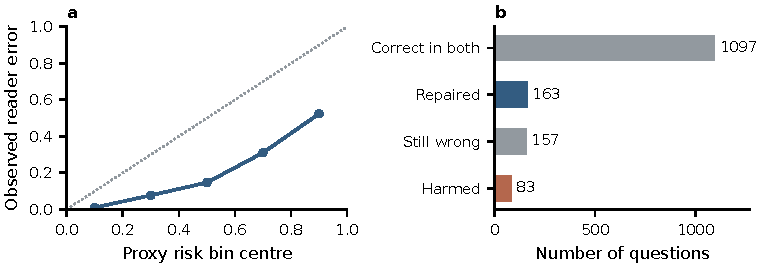
\includegraphics[width=.82\linewidth]{figs/stratification.pdf}
\caption{CUAD library validation with 300 questions per proxy risk bin and GPT-5.6-terra as reader. (a) Observed error rises with proxy risk. The dotted line marks equality, which the score does not attain because it ranks rather than estimates error. (b) Outcomes when the extracted contract definition is supplied. Repairs outnumber harms, and about half of the original errors remain.}
\label{fig:strata}
\end{figure}

\paragraph{What the score measures.}
$R$ also predicts errors that cannot be attributed to a conflicting local meaning. On synthetic terms retaining their usual meaning, its AUROC is 0.921 for DeepSeek V4 Flash and 0.846 for GPT-6-astra, based on 21 and 6 errors. On Reddit non-glossary controls it is 0.842 and 0.815 (Appendix~\ref{app:synthetic-control}). These controls make shared question difficulty a plausible component of the signal. The synthetic class comparison and definition interventions establish that local content matters in some questions, but $R$ alone cannot say \emph{why} a particular answer will be wrong. Its practical role is review triage, with the source definition and the question checked separately.

\paragraph{Question validity.}
Source-linked scores are only as credible as their keys. Two models screened 80 fixed-hash questions against available source material, after which an author reviewed 17 model-disagreement items and 10 stratified controls without seeing the keys. Subsequent source reconciliation classified 10 stored keys as supported, 14 questions as invalid or source-insufficient, and 3 as borderline. The selected 27 do not estimate a corpus-wide defect rate (Appendix~\ref{app:source-screen}, Table~\ref{tab:review}). Deleting the 14 clear problem items changes $R$ error AUROC by at most 0.00203 across the eight matched settings and leaves the synthetic 93/229 stable-error count unchanged. This local sensitivity says the \emph{found} problems do not drive those point estimates; it cannot validate unreviewed keys. We consequently treat synthetic and CUAD as the main controlled diagnostic evidence and Reddit and DeFi as exploratory transfers.

